\documentclass[titlepage]{article}
\usepackage[utf8]{inputenc}
\usepackage[spanish]{babel}

% Header
\usepackage{fancyhdr}
\pagestyle{fancy}
\fancyhf{}
\fancyhead[L]{Asier Sampietro Alberdi}
\fancyhead[R]{\leftmark}
\fancyfoot[R]{\thepage}

% Graficos
\usepackage{graphicx}
\graphicspath{ {images/} }

% Secciones
\makeatletter
\newcommand\level[1]{%
  \ifcase#1\relax\expandafter\chapter\or
    \expandafter\section\or
    \expandafter\subsection\or
    \expandafter\subsubsection\else
    \def\next{\@level{#1}}\expandafter\next
  \fi}
\newcommand{\@level}[1]{%
  \@startsection{level#1}
    {#1}
    {\z@}%
    {-3.25ex\@plus -1ex \@minus -.2ex}%
    {1.5ex \@plus .2ex}%
    {\normalfont\normalsize\bfseries}}

\newdimen\@leveldim
\newdimen\@dotsdim
{\normalfont\normalsize
 \sbox\z@{0}\global\@leveldim=\wd\z@
 \sbox\z@{.}\global\@dotsdim=\wd\z@
}

\newcounter{level4}[subsubsection]
\@namedef{thelevel4}{\thesubsubsection.\arabic{level4}}
\@namedef{level4mark}#1{}
\def\l@section{\@dottedtocline{1}{0pt}{\dimexpr\@leveldim*4+\@dotsdim*1+6pt\relax}}
\def\l@subsection{\@dottedtocline{2}{0pt}{\dimexpr\@leveldim*5+\@dotsdim*2+6pt\relax}}
\def\l@subsubsection{\@dottedtocline{3}{0pt}{\dimexpr\@leveldim*6+\@dotsdim*3+6pt\relax}}
\@namedef{l@level4}{\@dottedtocline{4}{0pt}{\dimexpr\@leveldim*7+\@dotsdim*4+6pt\relax}}

\count@=4
\def\@ncp#1{\number\numexpr\count@+#1\relax}
\loop\ifnum\count@<100
  \begingroup\edef\x{\endgroup
    \noexpand\newcounter{level\@ncp{1}}[level\number\count@]
    \noexpand\@namedef{thelevel\@ncp{1}}{%
      \noexpand\@nameuse{thelevel\@ncp{0}}.\noexpand\arabic{level\@ncp{1}}}
    \noexpand\@namedef{level\@ncp{1}mark}####1{}%
    \noexpand\@namedef{l@level\@ncp{1}}%
      {\noexpand\@dottedtocline{\@ncp{1}}{0pt}{\the\dimexpr\@leveldim*\@ncp{5}+\@dotsdim*\@ncp{0}\relax}}}%
  \x
  \advance\count@\@ne
\repeat
\makeatother
\setcounter{secnumdepth}{100}
\setcounter{tocdepth}{100}
% Secciones end

\setlength{\parskip}{1em}

\begin{document}
\begin{titlepage}
  \centering
  
\includegraphics[scale=0.35]{titulo1} \\
  \vspace*{1cm}
  \huge
  Máster Universitario en Tecnologías de la Computación Aplicadas al Sector Financiero\par
  \LARGE
  Curso académico 2018/2019\par
  Memoria de Prácticas académicas en empresa\par
  \Large
  \raggedright
  Título: Desarrollo y mantenimiento del aplicativo FIT\\
  Empresa: Almis Informática Financiera, S.L.\\
  Tutor en la empresa: José Manuel Núñez Fernández\\
  Tutor académico en la Universidad:  María Paula De Toledo Heras\\
  14 de Julio de 2019\par
  \centering
  
\includegraphics[width=\textwidth]{titulo2}\\


\end{titlepage}

\section*{Resumen del trabajo}
El trabajo realizado en Almis Informática Financiera S.L. (referido como Almis en adelante) ha tratado sobre la ampliación de las funcionalidades de una aplicación financiera. En concreto, se ha trabajado en el apartado de tratamiento de eventos sobre renta variable que dispone la ampliación. En el documento se detallarán los siguientes apartados: definición del problema, las actividades realizadas, las conclusiones y las competencias trabajadas.
\newpage

\tableofcontents
\newpage
\listoffigures
\newpage

\level{1}{Definición del problema}
La aplicación principal de Almis (en adelante referido como FIT, Financial Intelligence Tool) es un gestor de carteras usado mayormente para gestionar carteras en agencias de valores. Esta aplicación cuenta con numerosas herramientas usadas día a día por gestores, pero es una herramienta que sigue en desarrollo. Las principales necesidades de FIT son labores de desarrollo y de mantenimiento.\par

El apartado del desarrollo esta enfocado de cara a cliente. Este manda peticiones y se desarrollan soluciones a medida o globales, que podrían interesar a otros usuarios. Aunque las peticiones tienden a ser variadas y se opte por hacerlas a medida, el último año se han centrado en funcionalidades sobre los eventos de renta tanto fija como variable.\par

El apartado de mantenimiento, en cambio, se centra en el departamento de QoS\footnote{\emph{Quality of Service}. Del inglés, ofrecer un servicio de calidad.}. FIT es una herramienta que ha crecido mucho, y a medida que se añaden procesos, el cómputo general se ralentiza cada vez más. Esto provoca una mala experiencia de usuario, y en FIT se trabaja para que esto suceda lo menos a menudo posible.

\level{2}{Desarrollos}
La demanda de este año ha ido enfocado a un robusto módulo de gestión de eventos. Los clientes quieren automatizar cada vez más eventos relacionados principalmente con la renta variable. Debido al aumento de inversores de pequeña escala gracias a las aplicaciones de trading, los clientes se enfrentan a una demanda mayor de eventos sobre las acciones de los clientes.\par

Estos desarrollos, al ser principalmente cálculos realizados cuando las carteras pasan de día\footnote{Cuando una cartera pasa de día se calculan los resultados de las operaciones que vencen a dicha fecha, y se actualiza su posición en base a ello.}, se componen de tareas relacionadas con el back-end\footnote{Parte de la aplicación web que no visible, encargado de cálculos y gestión de los datos.}, siendo el front-end\footnote{Parte de la aplicación web que visualiza el usuario, con una carga lógica mínima.} casi idéntico. Por este motivo, plantea añadir los nuevos eventos a una ventana web ya en uso para eventos similares.\newpage

\level{3}{Eventos}
Tras reuniones con clientes, se ha optado por priorizar 3 eventos, uno de los cuales necesita ser mejorado y otros dos que deben ser desarrollados desde cero.

\level{4}{Derechos de suscripción}
Este evento es el que esta desarrollado parcialmente. La implementación se hizo para salir del paso en su momento, y ahora se quiere mejorar porque el uso ha aumentado.\par

Este evento sucede cuando una empresa decide hacer una ampliación, para evitar que el porcentaje de participación de un accionista caiga o diluya. Para ello, los accionistas cambian sus posiciones a derechos. De esta manera, tienen una posición temporal mientras se amplia el capital. Al terminar, los derechos se transforman de nuevo en acciones, en este caso en las nuevas acciones, con el porcentaje que tendría el accionista en el estado actual. Los derechos de suscripción son instrumentos comerciables. Se pueden vender en el mercado como si fueran acciones; recibir dividendos; o venderlos al emisor, que es en lo que se diferencian principalmente a las acciones.\par

Y es este caso de uso el que necesita adoptar FIT. Actualmente el emisor de los derechos no puede establecer un precio al cual se venderán las acciones de los interesados en una fecha dada, por lo que se requiere un desarrollo sobre el código que ya está en producción. Aprovechando esto, también se retocara la ventana, ya que como se ha mencionado anteriormente, se hizo con poco detalle para salir de paso.


\level{4}{Primas de asistencia}
También relacionado con los accionistas, el segundo evento a tratar son las primas a los asistentes de las juntas de accionistas. El emisor de este evento definirá un precio que pagara por cada acción que posea el asistente.\par

Al tratarse de un evento simple (a nivel de interfaz), se piensa incluir en la ventana de pagos y cobros. Esta ventana es la encargada de gestionar diferentes fluctuaciones en las posiciones de las carteras gestionadas. Cuando se crea un evento como este, se valida o rechaza desde esta ventana, creando así el flujo de caja correspondiente.\newpage

\begin{figure}[h]
\centering
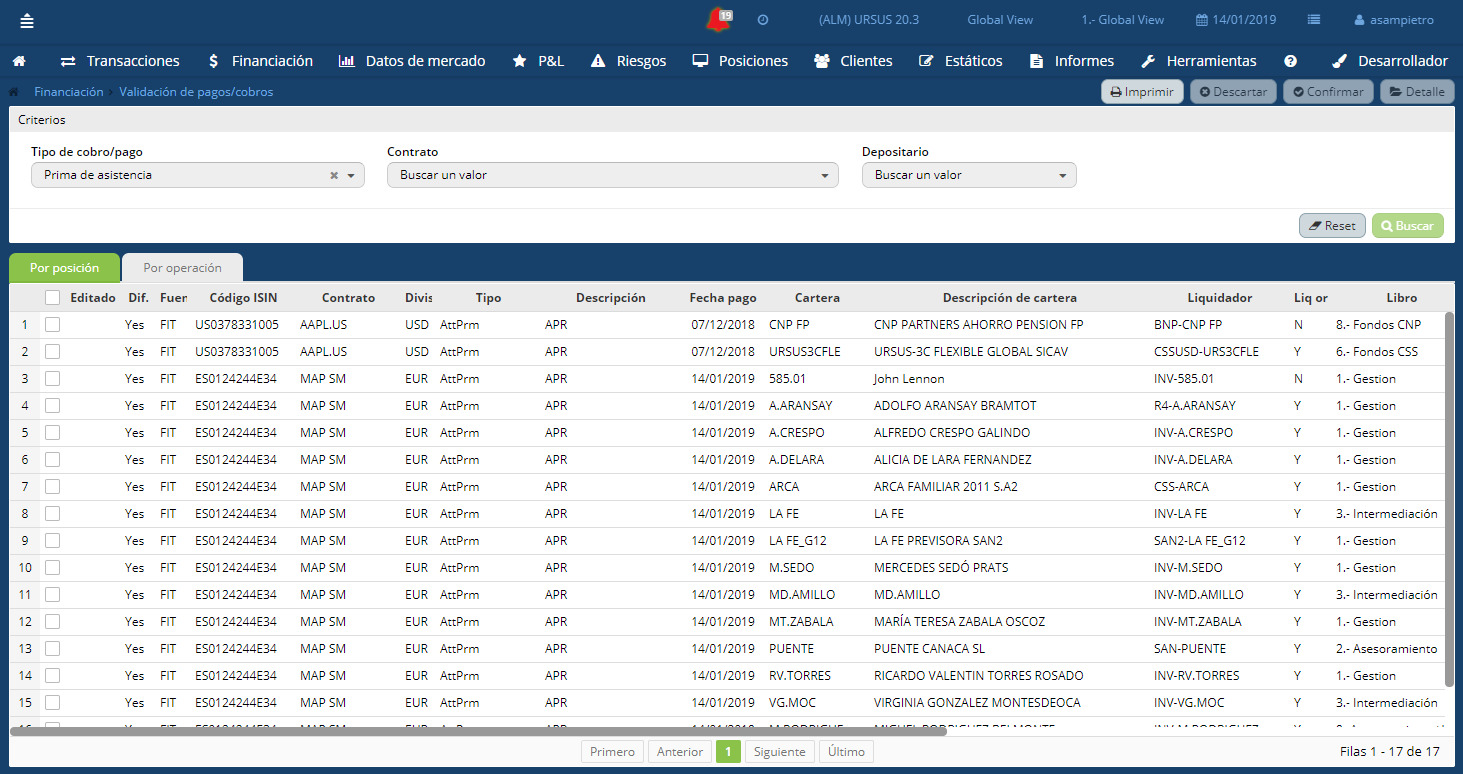
\includegraphics[width=\textwidth]{cobros_pagos}
\caption{Ventana de pagos y cobros}
\end{figure}

Como se puede observar en la figura 1, la ventana cuenta con un selector de eventos (o cobro o pago, como se le llama en la ventana), y puedes seleccionar varios para confirmarlos de una tacada. Desde el botón de 'Detalle' se pueden hacer ligeras modificaciones previas a la confirmación. También existe la posibilidad de descartarlos, rechazando la propuesta de la aplicación y teniendo que meterlo de forma manual posteriormente.

\level{4}{Prima de emisión}
Relacionado con los derechos de suscripción, los clientes también solicitan la posibilidad de ejercer una prima de emisión a la hora de darse una ampliación de capital.\par

La prima de emisión es la parte de la aportación que hay que realizar para suscribir una acción o participación que viene dada por diferencia entre su valor de emisión y su valor nominal. En otras palabras: la prima de emisión es la cantidad que hay que pagar para adquirir una acción o participación en el momento de su emisión además de su valor nominal. De esta manera, los accionistas más antiguos conservarán su ventaja manteniendo todos una parte equitativa de la empresa a lo aportado.\newpage

\level{2}{Tareas de mantenimiento}
FIT es una aplicación que no para de desarrollarse junto con el motor que le brinda un entorno web. La evolución de continua de estos dos hace que los apartados más viejos se vean realmente perjudicados, y por eso se deben hacer varias tareas de mantenimiento de manera constante para cumplir con la promesa de calidad con el cliente. Por ello se han marcado varias ventanas como candidatas a una refactorización.\par

Como se ha comentado anteriormente, el foco de este año ha ido fijado en los eventos sobre posiciones, y es por esto que se ha decidido mejorar varias ventanas relacionadas con estos.\newpage

\level{3}{Ventana de pagos y cobros}
La ventana anteriormente mencionada, cuenta con diversos eventos que requieren tratos específicos. Como se puede observar en la figura 2, la ventana cuenta con demasiados eventos como para dar un trato específico para cada uno de ellos, por lo que es necesario un trabajo de homogeneización.

\begin{figure}[h]
\centering
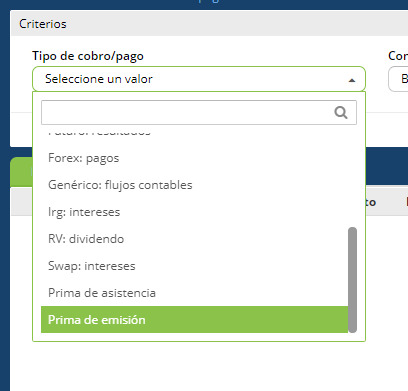
\includegraphics[scale=0.6]{tipo_cobros_pagos}
\caption{Eventos disponibles en la ventana de pagos y cobros.}
\end{figure}

Esta labor no cambiará nada a nivel visual, pero se encargará de brindar una navegación más agradable para el usuario.\newpage

\level{3}{Ventanas de definición de eventos de renta variable}
La filosofía de Almis respecto al reciclaje de código ha sido el causante de esta necesidad. Como todos los eventos se declaran de manera similar. Siguiendo el afán de reutilización, se optó por crear una ventana genérica para todos los eventos, y gestionar mediante dependencias\footnote{Eventos de la ventana que desecadenan acciones.} de AngularJS\footnote{Un motor desarrollado en JavaScript que permite dinamizar las ventanas web.} las diferencias que podían darse, añadiendo coste computacional al navegador.\par

Llegados a cierto punto, esta estrategia ha resultado inviable, puesto que ciertos clientes (debido a la multitud de datos que cotejan) son incapaces de gestionar nada mediante estas ventanas, ya que el navegador no soporta tal carga.\par

A son de este problema, se ha optado por dividir la ventana base en múltiples, tratando cada evento desde la ventana misma y reduciendo las inyecciones de AngularJS.\par

\begin{figure}[h]
\centering
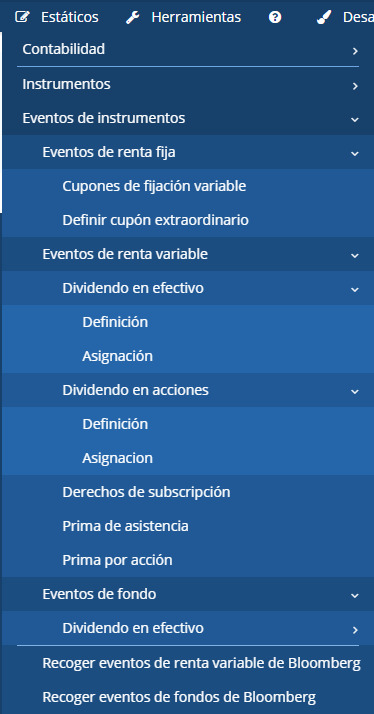
\includegraphics[scale=0.3]{ventanas_optimizadas}
\caption{Menú con las ventanas optimizadas.}
\end{figure}

Como se puede observar en la figura 4, todas estas ventanas parten de la misma base. Se duplicará el código y se modificará cada caso para habilitar estas ventanas al uso de nuevo.

%---------------------------------------------------------

\level{1}{Actividades realizadas}
Para enfrentarse al problema descrito, se han realizado las siguientes tareas en los ámbitos de desarrollo y mantenimiento de la aplicación.

\level{2}{Desarrollo de eventos}
Como se ha mencionado anteriormente, dentro de todos los eventos que recoge o plantea recoger FIT, se ha puesto el foco en tres. Estos son los desarrollos que se han realizado para cada uno para ofrecer una solución a las necesidades de los clientes.\par

\level{3}{Primas de asistencia}
La gestión de las primas de asistencia ha sido desarrollada desde cero. Como se ha mencionado en el planteamiento del problema, la ventana de pagos y cobros ha sido la elegida de albergar esta funcionalidad, así que lo primero que se ha hecho es compatibilizar la tabla de la base de datos que refleja esta ventana.\par

Los datos se separan en dos tablas: una que recoge los datos generales del evento, como fecha de vencimiento, importe de la prima o datos del emisor; y otra que guarda temporalmente los detalles del evento y se calcula y rellena en tiempo de ejecución.\par

\begin{figure}[h]
\centering
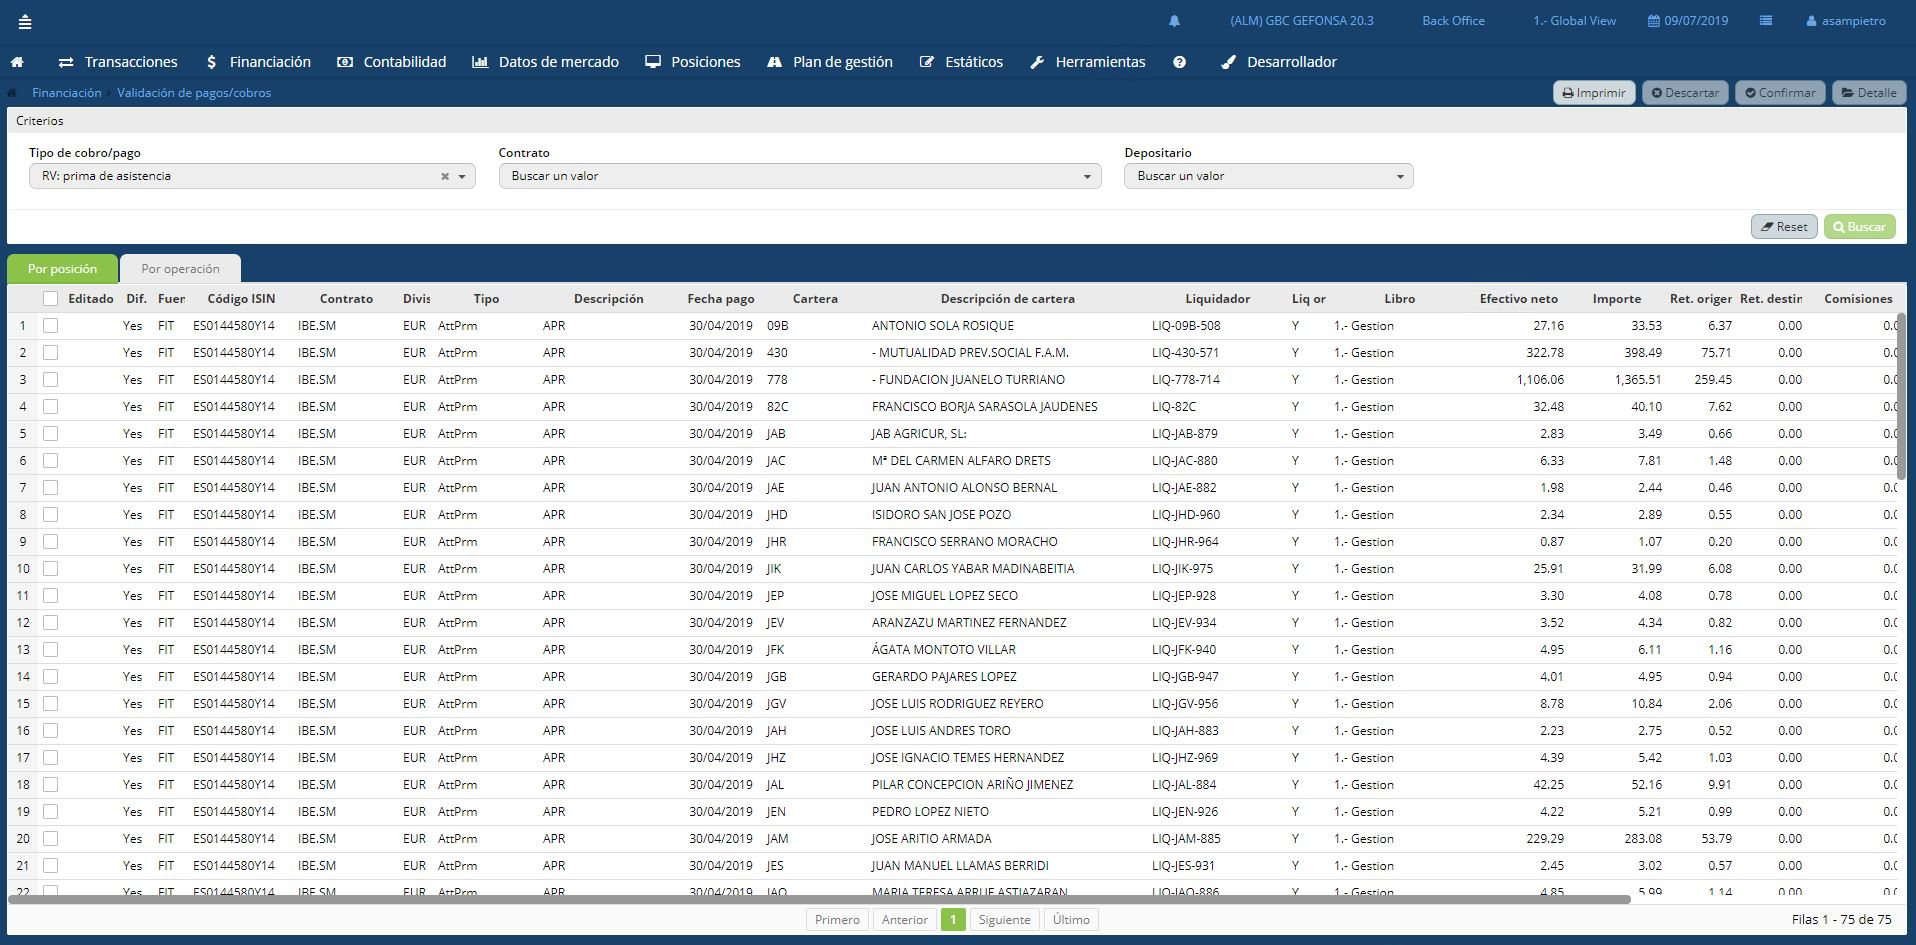
\includegraphics[width=\textwidth]{primas_asistencia}
\caption{Listado de primas de asistencia.}
\end{figure}

Tras validar que ambas tablas son aptas para el desarrollo, se ha pasado a la parte de visualización. Como se ha mencionado, la visualización conlleva una serie de cálculos que ofrecen detalles sobre el evento, como retenciones y comisiones, junto con el efectivo neto. Se ve más claro en el ejemplo de las figuras 4 y 5.\par

\begin{figure}[h]
\centering
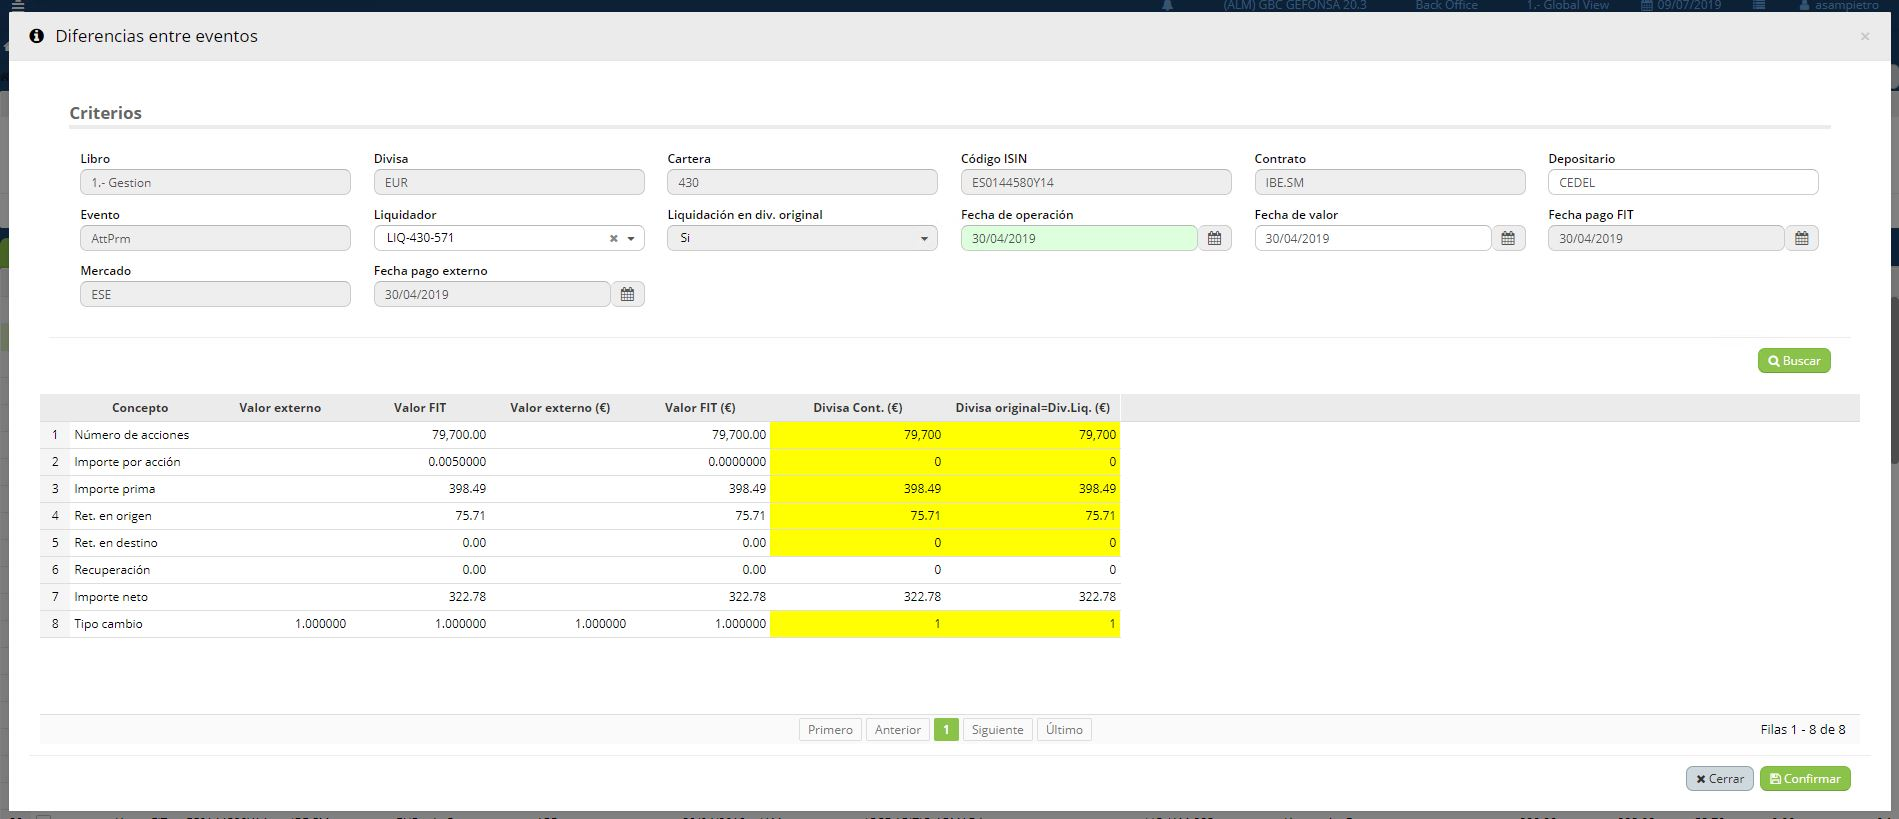
\includegraphics[width=\textwidth]{detalle_primas_asistencia}
\caption{Detalles de las primas de asistencia.}
\end{figure}

Una vez conseguido visualizar los datos, se pasa a la ejecución o confirmación del evento. Esto se realiza mediante una función de C donde se calculan los flujos que va a generar esta operación, y se dejan almacenados en una tabla de la base de datos. Esto se hace así porque los resultados se calculan al final del día, junto con el resto de cálculos.\par

La teoría de este calculo es el siguiente: se parte de la prima, y se recogen todas las posiciones de una cartera; se multiplica para saber el bruto, y de ese bruto se extraen las retenciones que tendrá para calcular el neto, por ultimo, con los demás datos se crean los flujos de caja y se almacenan en la base de datos.\par

Al igual que un cobro se puede aceptar, también se tiene que poder cancelar, así que también se necesita esa implementación. Esta parte del desarrollo es bastante más sencilla debido al modelo de datos. Simplemente se almacena toda la información para posterior auditoría, y se marca como cancelado en la base de datos.\par

Por último, el principal funcionamiento para esta ventana es que los eventos sean confirmados en masa así que es común tener que deshacer alguno. Por lo tanto, se ha desarrollado una ventana que recoge la información del evento confirmado. En la figura 6 se puede observar como es la ventana para dicho funcionamiento. El proceso es parecido a la confirmación, solo que se mete un flujo inverso para neutralizar el anterior. Esto cuando se realice la liquidación será transparente.

\begin{figure}[h]
\centering
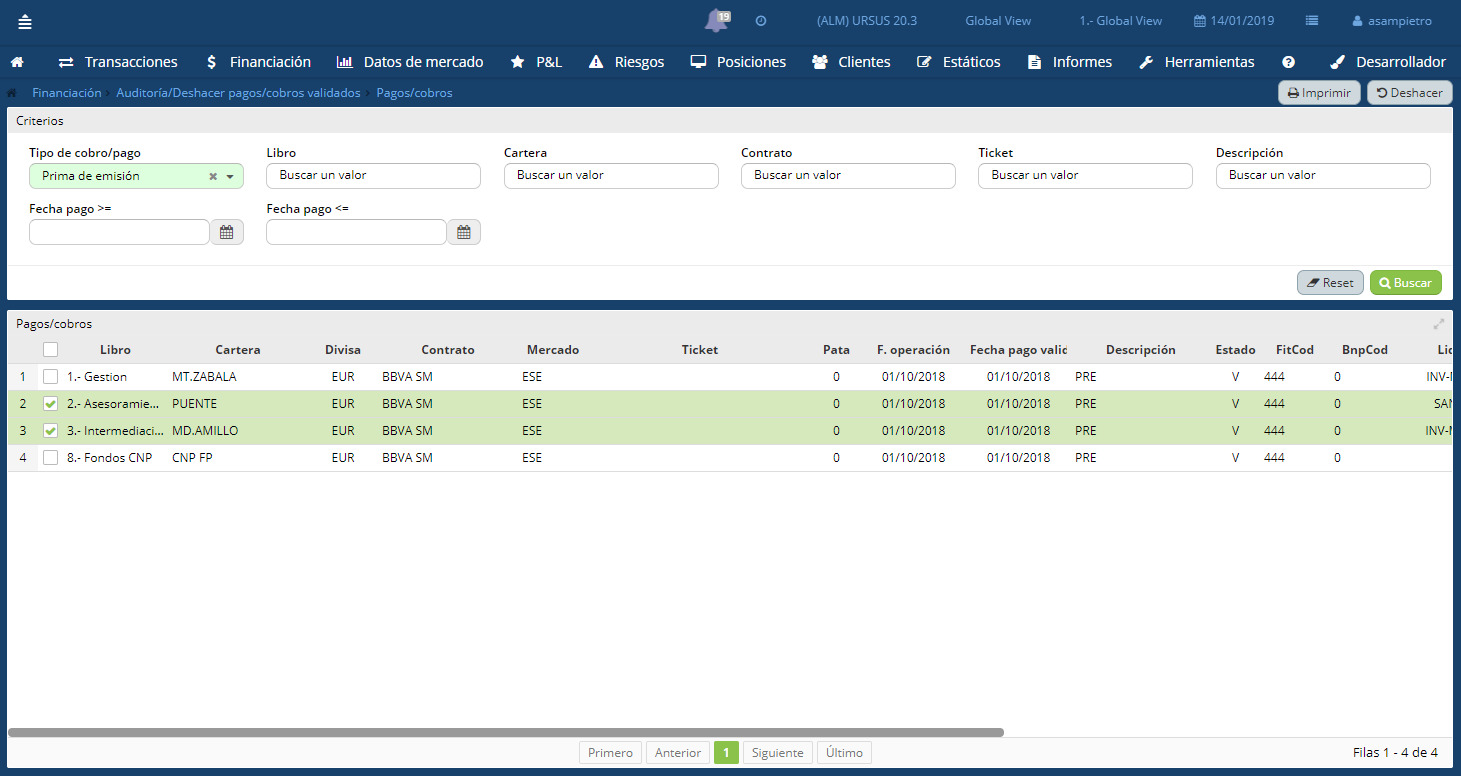
\includegraphics[width=\textwidth]{auditoria}
\caption{Auditoría del cobro, y botón de deshacerlo.}
\end{figure}
\newpage

\level{3}{Primas de emisión}
Las primas de emisión son muy parecidas a las primas de asistencia, computacionalmente. Como se ha mencionado en el planteamiento del problema, se ha metido también en la ventana de cobros y pagos, por motivos similares a las primas de asistencia.\par

A nivel visual, la única diferencia que encontramos con las primas de asistencia es que estas no llevan ningún tipo de retención, por lo que la ventana de detalle es mas simple que los anteriores eventos.\par

También dispone de una ventana de auditoría, en la que se pueden deshacer las confirmaciones, ya que estos también están pensados para ser confirmados en masa.\newpage

\level{3}{Derechos de suscripción}
La parte de derechos de suscripción que se ha tenido que desarrollar es el llamado 'scrip dividend', o dividendo opcional. Cuando se desea realizar una ampliación de capital, la entidad emisora da la opción de comprar todos los derechos que no se deseen, para facilitar la venta a sus accionistas. De esta manera, y por un precio fijado, se apropia de derechos que luego venderá como nuevas acciones para acaparar más accionistas.

La ventana actual de los derechos de suscripción cuenta con dos botones para la asignación y conversión, así que se añade uno nuevo para la venta, como se observa en la figura 7.

\begin{figure}[h]
\centering
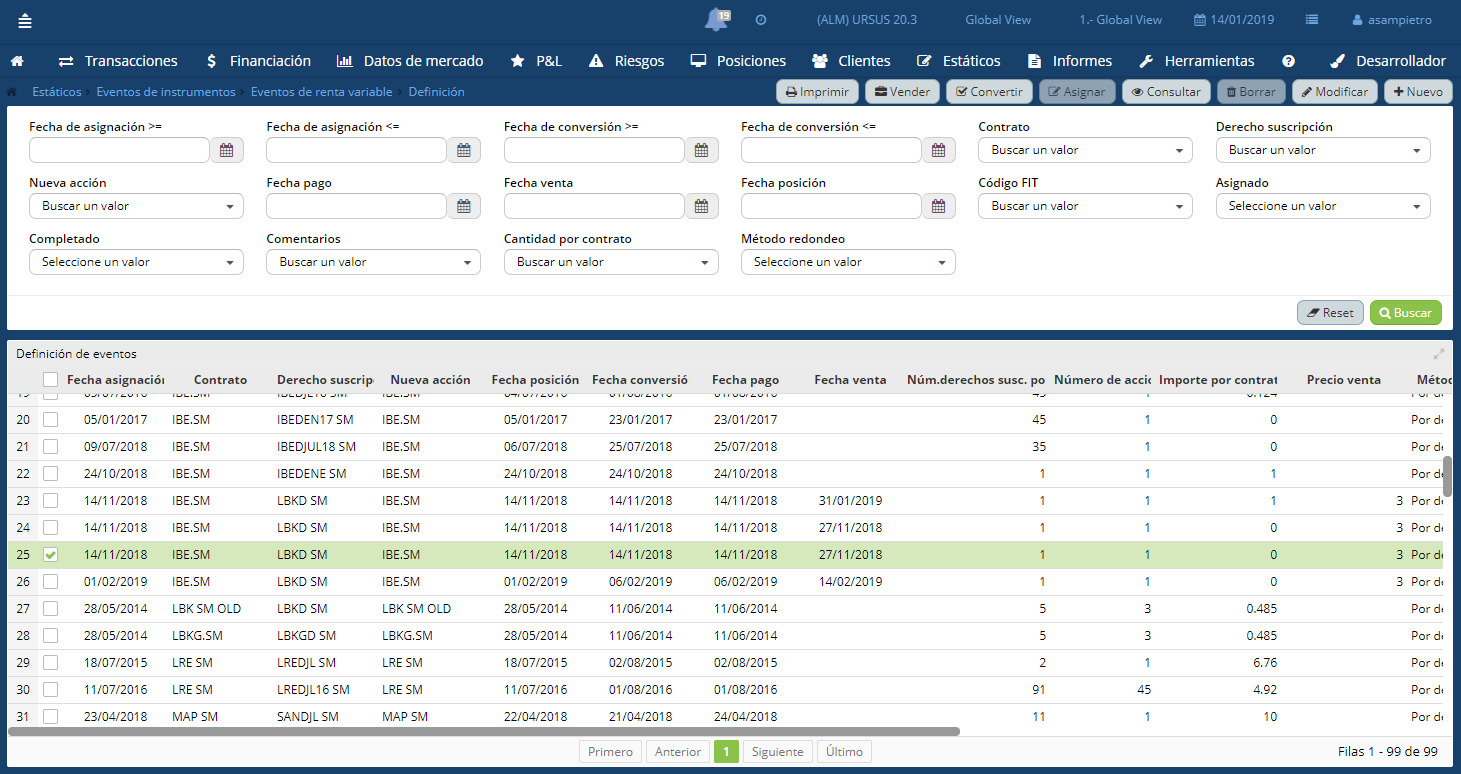
\includegraphics[width=\textwidth]{derechos_suscripcion}
\caption{Ventana de gestión de derechos de suscripción.}
\end{figure}

\newpage
A parte de esto, también se deben crear nuevos campos en el dialogo de creación, ya que el usuario puede definir el precio indicado por la empresa emisora. Con los nuevos campos quedaría de la manera que se ve en la figura 8.

\begin{figure}[h]
\centering
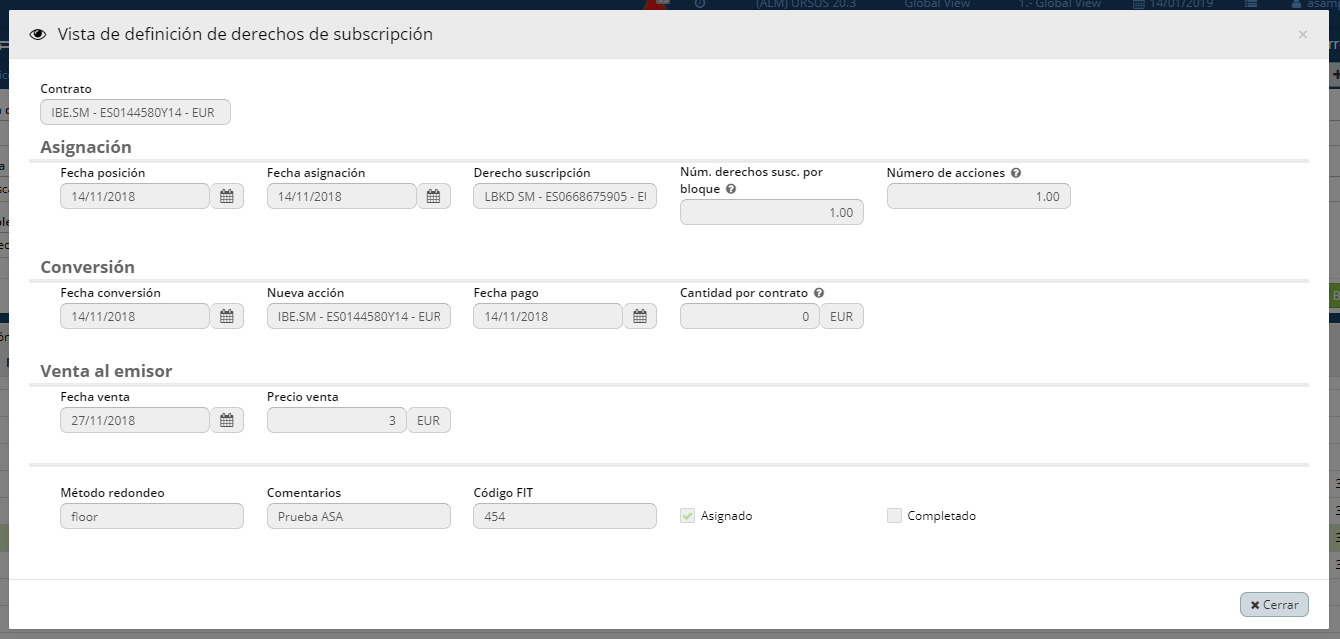
\includegraphics[width=\textwidth]{definicion_derechos_suscripcion}
\caption{Creación de derechos de suscripción.}
\end{figure}

La venta al emisor se ha desarrollado siguiendo el ejemplo de la conversión. A nivel algorítmico, la conversión trata de una venta a precio 0 de los derechos, y una compra a precio 0 de las nuevas acciones. Lo que se ha hecho para esta nueva funcionalidad ha sido coger la venta de derechos y añadirle el precio. Con esto, similar a los otros dos eventos, se genera un flujo de caja que se liquida mediante batches\footnote{Scripts escritos en el lenguaje batch de Windows para ejecuciones automatizadas} nocturnos.\par

Para realizar este desarrollo, se ha tenido que tocar también la parte de las conversión, ya que la funcionalidad actual solo permitía la confirmación en masa, sin dar opción a elegir que se quería convertir y que no. Ahora se pueden seleccionar las líneas que quieras convertir o vender.
\newpage

\level{2}{Optimización de ventanas}
La optimización de ventanas también ha ido enfocado al modulo de eventos, código que se ha tocado anteriormente. El problema es similar en los dos casos que se han tratado: el afán por reutilizar ha acabado sobrecargando la ventana.

\level{3}{Ventana de cobros y pagos}
Como se viene diciendo en todo el documento, esta ventana tiene demasiadas eventos gestionados de manera similar. Tanto la interfaz gestionada por AngularJS, como el back-end de C esta demasiado saturado de bombas lógicas\footnote{Se refiere a bomba lógica cuando dos instrucciones se contradicen y su comportamiento no esta definido} que ralentizan los procesos.\par

Para dar mas agilidad a las ventanas, se ha pasado por un proceso de detección de cuellos de botella. Se han añadido marcas temporales en los procesos para identificar las zonas más lentas. También se ha hecho una inspección de trazas web para detectar bombas lógicas, detectando casi un centenar de ellas.\par

Primero se ha procedido a limpiar la interfaz web, simplificando y unificando dependencias que se han ido añadiendo en cada desarrollo, desde un punto de vista mas global. Esto pese a ser relativamente simple, ofrece ya una mejora notable consiguiendo una navegación más fluida y menor carga de navegador. Además, se puede contrastar fácilmente con testeos de interfaz.\par

Después, se ha procedido a modificar el algoritmo, ya que gracias a las mediciones se han detectado bucles y cargas de datos innecesarios. El principal objetivo ha sido reducir peticiones a la base de datos. Optimizando bucles y reduciendo las lecturas y escrituras se ha conseguido acelerar en un 15\% el calculo.\newpage

\level{3}{Ventanas de definición de eventos de renta variable}
Estas ventanas parten todas de la misma raíz, y se llenaban de dependencias partiendo de un identificador que se cargaba al cargar la página. Esto causaba que todas las dependencias saltasen a la vez y el navegador no respondiera por quedarse sin memoria. Para evitar esto, se ha creado una página para cada uno de los eventos afectados. Se ha leído la definición del evento y que es lo que necesita, para eliminar y reducir las dependencias a las mínimas. Las ventanas han vuelto a ser usables gracias a la especificación.\newpage

\level{1}{Competencias generales el máster}
Realizando estas prácticas, se han obtenido las siguientes competencias:
\begin{itemize}
  \item Mercados Financieros:
  \begin{itemize}
    \item Al desarrollar funcionalidades para distintos tipos de eventos de renta variable, se ha adquirido conocimiento sobre los cálculos que se realizan para valorar dichos eventos.
    \item Al descomponer eventos para separar ventanas, se ha adquirido conocimiento sobre componentes de eventos de renta variable.
  \end{itemize}
  \item Tecnologías Aplicadas a los Mercados Financieros:
  \begin{itemize}
    \item Se han realizado mediciones de tiempos y análisis de cuellos de botella, y se ha aprendido a solventarlos.
    \item Se ha comprendido la diferencia de coste de lecturas a memoria o bases de datos.
  \end{itemize}
  \item Desarrollo de Software Financiero:
  \begin{itemize}
    \item Se ha comprendido las necesidades de escalabilidad que tiene el software financiero, al ver a la cantidad de carga que se enfrenta.
    \item Se ha obtenido una visión de lo que es trabajar en una aplicación financiera con varios grandes módulos.
  \end{itemize}
\end{itemize}
\newpage

\level{1}{Conclusiones}
Con este trabajo se ha tenido la primera toma de contacto con el mundo financiero, y partiendo de eso se han sacado las siguientes conclusiones referentes al apartado técnico tanto como a lo metodológico.
\level{2}{Conclusiones técnicas}
Referente a lo técnico, se han cumplido los objetivos planteados.\par

Se quería dar un impulso al modulo de eventos, y se han añadido 3 nuevas funcionalidades que complementan los ya presentes. Con esto la aplicación es cada vez más independiente y sin necesidad de terceros, camino a dar una solución más completa.\par

También se ha conseguido optimizar ciertos apartados, dando confianza al cliente de manera que vea mejoría constante. Siendo ventanas usadas constantemente, el poder ahorrar minutos de trabajo es algo que las empresas lo suelen agradecer.

\level{2}{Conclusiones metodológicas}
Respecto a la metodología, se ha visto un claro ejemplo de obsolescencia en cuanto a reglas, estilos y metodología de desarrollo. La falta de planificación en un pasado ha acarreado graves problemas a día de hoy.\par

Por ello se ha puesto un especial foco en conseguir soluciones robustas y no hacer chapuzas para salir de paso. Todo le que se ha generado ha ido estrictamente justificado y documentado, para evitar futuros problemas de este calibre.\par

\newpage
\level{1}{Bibliografía}
\begin{itemize}
  \item Almis Informática Financiera S.L., 1994. FIT. [En línea] \\ Disponible en: http://www.almis.com/es/tesoreria
  \item Almis Informática Financiera S.L., 1994. FIT FMB. [En línea] \\ Disponible en: http://demo.almis.com/FMB\_V0.0
  \item Almis Informática Financiera S.L., 2016. AWE Wiki. [En línea] \\ Disponible en: https://git.almis.com/awe-team/awe/wikis/home
  \item Almis Informática Financiera S.L., 2016. Selenium IDE Wiki. [En línea] \\ Disponible en: https://git.almis.com/awe-team/awe/wikis/selenium-3.1
\end{itemize}
\end{document}
